%
% File: chap01.tex
% Author: Liam O'Shea
% Description: Introduction chapter where the boxing goes.
%
\let\textcircled=\pgftextcircled
\chapter{Background \& Research}
\label{chap:intro}

\initial{T}his chapter describes and explains boxing concepts which are important to understanding the goal of the project. It gives an overview of the types of punches a boxer must execute along with common errors associated with those. It also reviews relavant literature in areas covered by this thesis and explores the current cutting edge possibilities.

%=======
\section{Boxing Background}
\label{sec:sec01}

Boxing requires an incredible amount of co-ordination and timing as well as the ability to rapidly execute punches in a controlled and precise manner. Unlike professional boxing which is 12 x 3 minute rounds an amateur bout is 3 x 2 minute rounds which changes the dynamics of the contest. Amateur boxing relies on a points scoring system since there is often insufficient time for knockouts. therefore amateur boxers rely on the mastery of technique and proper form. Dropping you hand for a split second can open you up to an experienced boxer and could spell disaster.

As someone who has boxed for over 5 years and captain of the university boxing club I know how difficult it is to develop good technique and also how much time and experience is required from a coach to develop a new boxer. This one-on-one time is incredibly valuable, expensive and hard to come by. My aim is to be able to identify different types of punches and to offer some sort of quality metric as well as feedback advice. This will bring some much needed expert advice to a beginner who can practice in the comfort of their own home.

This could be especially useful for the university club since we get new waves of people every year who have never boxed before. 

Maybe note here how IT IS NOT A KINECT BOXING GAME.

\subsection{Motivation}
\label{subsec:subsec01}

Every year the Amateur boxing club taking in new members that are total beginners. We spend an enormous amount of time and effort helping them learn the basics and encourage people to practice at home. The problem is that it’s incredibly hard to spot your own faults. If it was possible to practice at home with the benefits of coaching it would bring massive improvements to their abilities. It could also be used as a platform think it would be a great way to introduce younger children to the sport since the Xbox/Kinect is incredibly popular and so it’s great from an inclusion perspective.
I also have several years of coaching experience to call upon and an array of local talent who would be able to offer advice if needed.

\section{Boxing Technique}
\label{sec:sec02}
For the scope of this project I am going to focus on the most common orthodox stance. There are tens of slight variations on each punch but I am going to focus on the core and important principles from which these can be built.

\subsection{Stance}
\label{subsec:subsec02}
The most fundamental building block of boxing is the stance, that is how you hold and position your body as well as the placement \& orientation of your feet. A good stance is crucial since it allows the boxer to be well balanced and light on their feet, allowing fast movement in any direction as well as the ability to quickly duck, weave, slip and bob and lay back to avoid punches. It is also crucial for offense since the power from punches come from the transfer of weight from one leg to another which requires a very specific twisting hip movement. Often beginners forget this crucial step and so I'm hoping to use this unique trait to help me judge quality later on. A successful stance should have the following characteristics:

- Left foot forward, right foot back with the feet slightly wider than shoulder width with a 45 degree angle twist.
- Right heel of the ground at all times with weight placed more on your back leg
- Slightly bent knees
- Chin tucked down
- Right hand on the right hand side of your chin, left hand should be a few inches in front of the left side of the face
- Elbows tucked in

\subsection{Punches}
\label{subsec:subsec03}
\paragraph{Jab}
The elbow should stay tucked in while the left fist extends with palms facing inwards before twisting your wrist at the last moment. The natural thing to do is extend the punch with palms facing down, unfortunately this immediately makes the elbow stick out which allows the opponent to easily see you are about to throw a punch (telegraphing) while opening up your body for a counter attack.
The punch should also finish so your arm is fully extended which helps to extend your reach and protect your chin before speedily returning it to the guard position.
Characteristic to target: Sticking out elbow

\paragraph{Cross}
The cross is designed as your heavy straight punch and as such is slower but more powerful. To get a \'snappy\' and powerful punch it is important to transfer your weight rapidly from your back leg to your front leg. Right hand. Characteristic: Rapid and specific hip movement

\paragraph{Hooks}
Your elbow should come out so it is shoulder height and your fist and shoulder should be at 90 degrees to each other. Again a rapid transfer of weight between hips is needed. {\bf Characteristic: Rapid and specific hip movement}

\paragraph{Uppercuts}
This required the fighter to crouch down into the squat position and throw a punch vertically upwards, with the aim of striking the opponent's chin.
Characteristics: Crouch, directly vertical punch, keeping guard close at all times.\cite{Rector2013}

\section{Kinect}
This section provides some background information about Microsoft Kinect that is important
for understanding the features and limitations of Kinect Analysis.
According to Microsoft, the Kinect  has worldwide sales of approximately 28 million units and contains an RGB camera, an infrared (IR) emitter and an IR depth sensor as well as a multi-array microphone. The interaction space of the Kinect is limited by the field of view of the Kinect cameras. The Kinect has a 43 ◦ vertical by 57 ◦ horizontal field of view. The Kinect sensor can be tilted using a built-in tilt motor. Tilting the Kinect increases the interaction space by +27 and −27 degrees.
The Kinect sensor provides sensor data in form of data streams. It can capture audio, color
and depth data. In addition, it can process the depth data to generate skeleton data. Therefore, the Kinect offers four different data streams that can be accessed: audio stream, color stream, depth stream and skeleton stream.
The streams can deliver at most 30 frames per second (FPS) using a resolution of $640\times480$ which drops to 12 FPS with a resolution of $1280\times960$

\paragraph{Depth \& Infrared Stream}
The depth sensor generates invisible IR light to determine an object's depth from the sensor. The primary use for the IR stream is to improve external camera calibration using a test pattern observed from both the RGB and IR camera to more accurately determine how to map coordinates from one camera space to another. \cite{irstream} The NUI API uses the depth stream to detect the presence of humans in front of the sensor.\cite{winSDK} Skeletal tracking is optimized to recognize users facing the Kinect, so sideways poses provide some challenges because parts of the body are not visible to the sensor.

\subsection{Skeleton \& Joint Tracking}
The Kinects default tracking mode can track up to 20 joints per skelton providing the subject is standing relatively face on and are fully visible to the sensor. Although the Kinect is capable of different modes (e.g. sitting) this is not relevant in the context of my project.
Each skeleton frame contains the position of each joint as well as information about the tracking quality. Joints can have one of three different tracking states, Not Tracked (0), Inferred (1) and Tracked (2), this flag is useful as an indicator of the quality of the measurements you are receiving for a particular joint. When possible tracked joints are used to help calculate the position of those joints that cannot be directly tracked hence the inferred joints. The Kinects default tracking mode is designed to track people who are standing and fully visible to the sensor.  The default range requires skeletons to be at least 80 centimeters away from the device to be tracked properly.

\paragraph{Data Format}
I record data from the Kinect in a space separated text file with each line corresponding to one timeframe. The structure of a line is: 
tracking_flag x_0 y_0 z_0 tracking_flag x_1 y_1 z_1 ... tracking_flag x_19 y_19 z_19,
where x_i,y_i,z_i are the x,y,z coordinates representing the position of the ith joint.
Each new line is represented by a very large value that could not represent a Kinect measurement. (e.g. 2000000) 
The tracking_flag is an integer which describes the status of the joint:
Joint not tracked = 0, Joint position inferred = 1, Join position tracked = 2.
If the joint is not tracked the position is set to (-10000, -10000, -10000) and it should not be used.
The position of the camera is (0,0,0).


The joints are:
i=0: NUI_SKELETON_POSITION_HIP_CENTER
i=1: NUI_SKELETON_POSITION_SPINE
i=2: NUI_SKELETON_POSITION_SHOULDER_CENTER
i=3: NUI_SKELETON_POSITION_HEAD
i=4: NUI_SKELETON_POSITION_SHOULDER_LEFT
i=5: NUI_SKELETON_POSITION_ELBOW_LEFT
i=6: NUI_SKELETON_POSITION_WRIST_LEFT
i=7: NUI_SKELETON_POSITION_HAND_LEFT
i=8: NUI_SKELETON_POSITION_SHOULDER_RIGHT
i=9: NUI_SKELETON_POSITION_ELBOW_RIGHT
i=10: NUI_SKELETON_POSITION_WRIST_RIGHT
i=11: NUI_SKELETON_POSITION_HAND_RIGHT
i=12: NUI_SKELETON_POSITION_HIP_LEFT
i=13: NUI_SKELETON_POSITION_KNEE_LEFT
i=14: NUI_SKELETON_POSITION_ANKLE_LEFT
i=15: NUI_SKELETON_POSITION_FOOT_LEFT
i=16: NUI_SKELETON_POSITION_HIP_RIGHT
i=17: NUI_SKELETON_POSITION_KNEE_RIGHT
i=18: NUI_SKELETON_POSITION_ANKLE_RIGHT
i=19: NUI_SKELETON_POSITION_FOOT_RIGHT

Inference

\subsection{Literature Review}
The Kinect is currently a rich area of research in its own right and it straddles the fields of Image Processing and Computer Vision as well as Human computer Interaction which are exciting and popular areas of research. I wanted to see what was capable with the Kinect at the cutting edge of research so I made use of the Conference on Computer Vision and Pattern Recognition (CVPR), International Conference on Computer Vision (ICCV) \& European Conference on Computer Vision (ECCV) to find relevant and useful research. 
The Kinect has been used in several sporting applications to help improve learn \& improve poses. In 2013 a controlled study of 16 people who were blind or who had low vision was ran to test the usefulness of Eyes-Free Yoga: An Exergame Using Depth Cameras for Blind \& Low Vision Exercise. The purpose of this was to teach the participants yoga poses using audio feedback and a positive response from participants. This however did only show success using very slow and static movements and so did not help me evaluate if my goal was feasible. 
It has also been used to evaluate a dancers performance
It has also been used to recognise Karate movements and give a quality measurement on the movements performed to 

\section{Existing Products}
\paragraph{UFC Personal Trainer}
The closest commercial product is a game called \'UFC Personal Trainer\' which is a very broad commercial product aimed at introducing people to UFC. After evaluating this product it became clear to me that it’s main focus is  exercise regimes rather than technical fighting. Therefore it does not offer the preciseness or technical fighting focus that I require. In this game even technically wrong punches will still register.

\paragraph{Kinect sports boxing game}
This has very poor punch discrimination and does not require any sort of real boxing ability. The goal here is usually to punch towards the kinect controller as quickly as possible. It fails to recognise properly thrown hooks and uppercuts and translate those into the game. 

\paragraph{Fighers Uncaged}
This game has generally poor reviews from reviewers, with most complaints centering around the reliability of the Kinect to accurately measure fighting moves. \cite{gamerev1} `'When the fights actually start, pulling off moves becomes a series of desperate flails, trying to get the game to recognize your actions.''\cite{gamerev2} 
and `'The game fails to register most of the movements'', `'The idea was great for Kinect, but something went horribly wrong along the way. Kinect is supposed to register your every kick and punch, but it only catches about the half of them.'', `'the Kinect control is lazily implemented.''\cite{gamerev3}



%A figures matrix.
\begin{figure}[t!]
\centering
\begin{minipage}{3.3cm}
    \centering
    \subtop[]{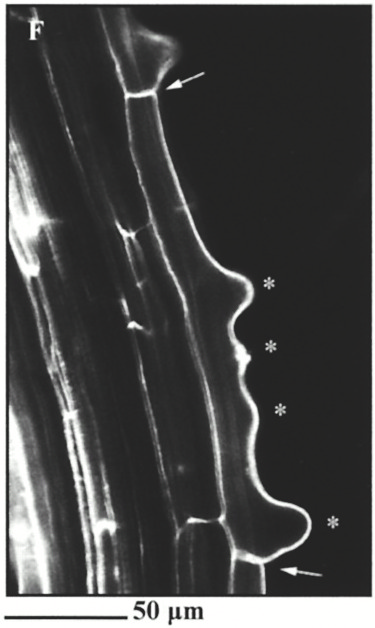
\includegraphics[height=0.28\textheight]{fig01/Nswellings}\label{sf:multiRH02a}}
\end{minipage}
\hspace{0.5cm}
\begin{minipage}{3.3cm}
    \centering
    \subtop[]{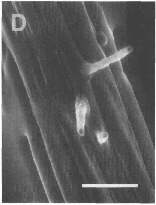
\includegraphics[height=0.27\textheight]{fig01/Mswellings}\label{sf:multiRH02b}}
\end{minipage}
\hspace{1.3cm}
\begin{minipage}{3.3cm}
    \centering
    \subtop[]{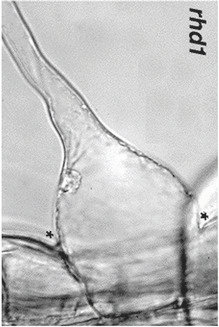
\includegraphics[height=0.27\textheight]{fig01/rhd1}\label{sf:multiRH02c}}
\end{minipage}
\\ \vspace{0.1cm}
\begin{minipage}{10cm}
    \centering
    \subtop[]{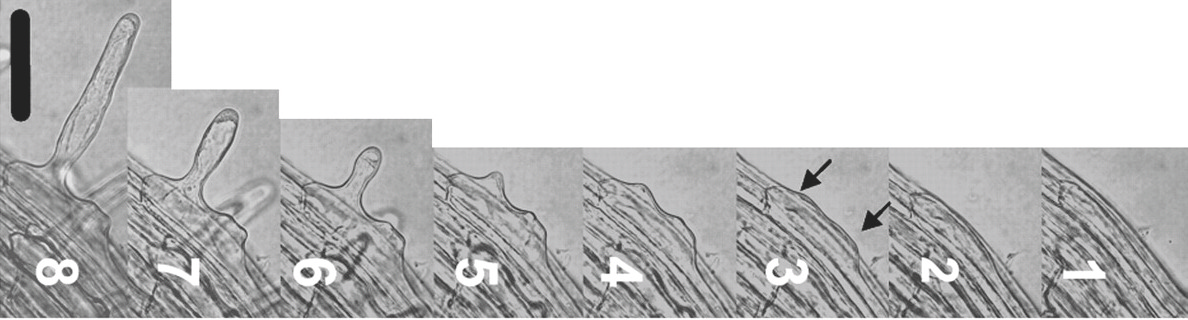
\includegraphics[height=0.145\textheight]{fig01/mutantrhd6}\label{sf:multiRH02d}}
\end{minipage}
\\ \vspace{0.1cm}
\begin{minipage}{10cm}
    \centering
    \subtop[]{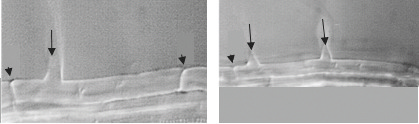
\includegraphics[height=0.16\textheight]{fig01/auxab}\label{sf:multiRH02e}}
\end{minipage}
\mycaption[Hair-forming mutant cells.]{(a) A mutant RH cell. Asterisks show multiple sites of RH initiation in a single root hair cell (indicated by the arrows). Figure reproduced from \cite{rigas01}. (b)~Hair-forming cell with three RH initiation locations. The bar represents $50\mu m$. Figure reproduced from \cite{massuci01}. (c) Large bump in mutant {\itshape rhd1}. Figure reproduced from \cite{griersonRH}. (d) Mutant overexpressing gene {\itshape ROP2}; from right-hand to left-hand, numbers indicate progressive snapshots at different times. RH initiation sites are indicated by the arrows. The bar represents $75\mu m$. Figure reproduced from~\cite{mjones01}. (e)~Mutants affected by auxin. On the left-hand side, RH site is farther away from the apical end (left arrow cap); on the right-hand side, multiple RH locations (arrows). Figure reproduced from~\cite{payne01}.}
\label{fig:multiRH02}
\end{figure}

% A single figure
\begin{figure}[t!]
	\centering
	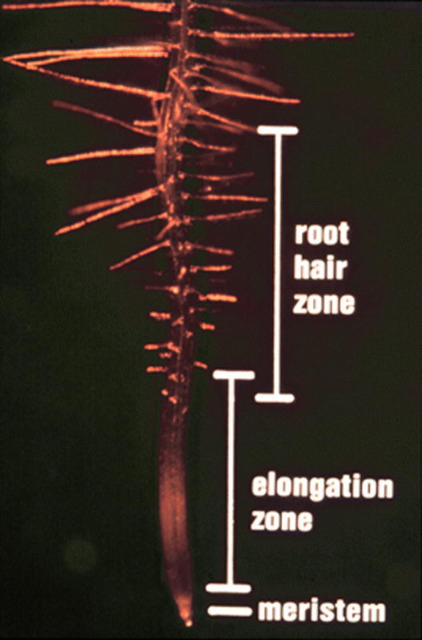
\includegraphics[height=0.35\textheight]{fig01/devepzones}
	\mycaption[Developmental zones of an Arabidopsis root.]{Developmental zones of an Arabidopsis root. Figure reproduced from \cite{griersonRH}.}
	\label{fig:RHP02}
\end{figure}

%=========================================================